\section*{Exercice 1}
\begin{wrapfigure}{r}{0.5\textwidth}
    \begin{center}
    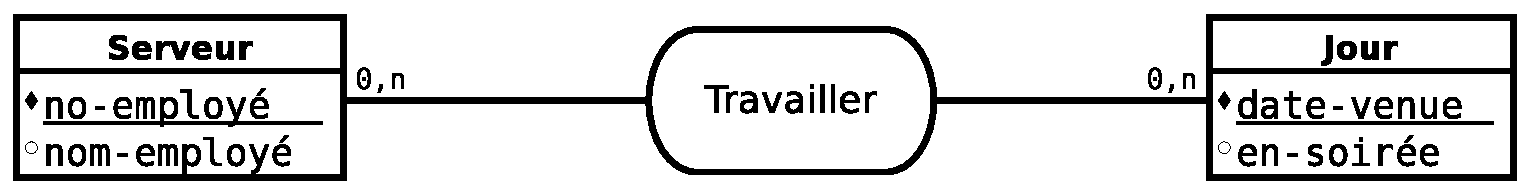
\includegraphics[width=0.4\textwidth]{partie_mcd.eps} 
    \caption{\label{mcd} Partie du MCD}
    \end{center}
\end{wrapfigure}
Un bar qui comptabilise le nombre de jour où ses serveurs travaillent en journée ou en soirée souhaite informatiser une partie de son système d'information. Un premier essai de modélisation a été effectué, mais le résultat ne correspond pas aux attentes. Déterminez ce qui ne va pas sur le MCD de la Figure~\ref{mcd} et apportez un correction sachant que : \\
\begin{itemize}
    \item Les serveurs peuvent choisir s'ils viennent la journée ou en soirée.
    \item Les serveurs peuvent changer leur choix chaque jour mais ne peuvent pas venir un même jour en journée et en soirée.
    \item Plusieurs serveurs peuvent venir pour le même service un même jour.
\end{itemize}

\section*{Exercice 2}
Le bar de l'Exercice~1, vous demande de continuer à modéliser son système d'information avec les contraintes suivantes : 
\begin{itemize}
    \item Les serveurs peuvent choisir s'ils viennent la journée ou en soirée.
    \item Les serveurs peuvent changer leur choix chaque jour mais ne peuvent pas venir un même jour en journée et en soirée.
    \item Plusieurs serveurs peuvent venir pour le même service un même jour.
    \item Pour savoir comment évaluer les salaires, le patron veut savoir sur une période donnée combien de clients sont servis en soirée et combien en journée.
    \item Il tient lui même les comptes de qui vient la journée et qui vient en soirée, mais veut que les salaires soient calculés automatiquement.
    \item Il souhaite également offrir une prime au serveur qui sert le plus de clients chaque mois, cela doit se faire automatiquement.
\end{itemize}

\subsubsection*{documents et données jugés utiles}
\begin{itemize}
    \item Ticket de caisse (numéro de ticket, numéro d'employé du serveur, date, nombre de clients)
    \item Fiche de paye (numéro d'employé, date de début de période, date de fin de période, nom de l'employé, salaire, prime)
    \item Livret des venues (nom du serveur, date des journées du mois, date des soirées du mois)
\end{itemize}

\subsubsection*{notes}
\begin{itemize}
    \item On ne s'occupe pas du détail d'une vente.
    \item Le résultat de l'Exercice 1 fait partie de la réponse.
    \item On ne gère pas l'organisation de l'emploi du temps.
\end{itemize}
